\chapter{Verification Techniques}
\label{ch:verif}

In the examples covered thus far, we have only used \uclid{} for bounded model checking of invariants. 
It can also be used to perform bounded model checking of linear temporal
logic properties.
In addition,
\uclid{} can be used to do unbounded inductive proofs and also provides support for debugging counterexamples. 
It can be used for checking simulation (refinement) between two transition systems,
such as the technique of correspondence checking between two
processor models.
Finally, \uclid{} can be used to check certain hyperproperties,
such as two-safety properties, by the technique of self-composition.
This chapter will describe these features of \uclid{}. Further features are being implemented and will be described in a future version of this document.

%---------------------------------------------------------
\section{Inductive Proofs} % change to \section when we have more sections!

Let us revisit the model from Example~\ref{ex:fib-model}. This is now shown again in Example~\ref{ex:fib-induction}, but with a different proof script. Instead of using the \codelike{bmc} command for bounded model checking, we are using the \codelike{induction} command to attempt an inductive proof.

\begin{uclidlisting}[htbp]
    \lstinputlisting[language=uclid,style=uclidstyle]{../examples/tutorial/ex4.1-fib-induction.ucl}
    \label{ex:fib-induction}
    \caption{\uclid{} Fibonacci model using induction in the proof script}
\end{uclidlisting}

\subsection{Debugging Counterexamples}

Let us try running \uclid{} on Example~\ref{ex:fib-induction} with the new proof script.
\begin{Verbatim}[frame=single, samepage=true]
$ uclid examples/tutorial/ex4.1-fib-induction.ucl 
Successfully parsed 1 and instantiated 1 module(s).
1 assertions passed.
1 assertions failed.
0 assertions indeterminate.
  FAILED -> induction (step) [Step #1] 
  property a_le_b @ ex4.1-fib-induction.ucl, line 14
Finished execution for module: main.
\end{Verbatim}

Uh oh, we seem to have a problem! \uclid{} is telling us that the inductive proof failed. We can try to examine why the proof failed by using the \codelike{print_cex} command to examine the counterexample to the proof.

\begin{uclidlisting}[htbp]
    \lstinputlisting[language=uclid,style=uclidstyle]{../examples/tutorial/ex4.2-fib-induction-cex.ucl}
    \caption{\uclid{} Fibonacci model with \codelike{induction} and \codelike{print_cex}}
    \label{ex:fib-induction-cex}
\end{uclidlisting}

The only changes between Example~\ref{ex:fib-induction} and Example~\ref{ex:fib-induction-cex} are on lines~18 and 21. \codelike{vobj} on line~18 is a reference to the verification conditions generated by the \codelike{induction} command. On line~21, we pass this reference to the \codelike{print_cex} command which prints out the values of \codelike{a} and \codelike{b} for the counterexample.

Running \uclid{} on Example~\ref{ex:fib-induction-cex} produces the following.

\begin{Verbatim}[frame=single, samepage=true]
Successfully parsed 1 and instantiated 1 module(s).
1 assertions passed.
1 assertions failed.
0 assertions indeterminate.
  FAILED -> vobj: induction (step) [Step #1] 
  property a_le_b @ ex4.2-fib-induction-cex.ucl, line 14
CEX for vobj: induction (step) [Step #1] 
property a_le_b @ ex4.2-fib-induction-cex.ucl, line 14
=================================
Step #0
  a : -1
  b : 0
=================================
=================================
Step #1
  a : 0
  b : -1
=================================
Finished execution for module: main.
\end{Verbatim}

To understand the counterexample, it is helpful to review how the inductive proof engine works. When inductively proving the \keyword{invariant} \codelike{a_le_b}, \uclid{} considers some arbitrary state that satisfies this property, executes the \keyword{next} block, and checks whether \codelike{a_le_b} holds on the resultant state.

The counterexample shows us that we do start in a state where $\codelike{a} \le \codelike{b}$ with $\codelike{a}=-1$ and $\codelike{b}=0$. We execute the \keyword{next} block and now \codelike{a} gets the value of \codelike{b}, becoming 0 and \codelike{b} gets the value $\codelike{a} + \codelike{b}$, becoming -1. This new state does not satisfy the invariant!

What is the real problem here? Taking a closer look at Example~\ref{ex:fib-induction-cex}, we see that this specific counterexample can never occur in our model because \codelike{a} and \codelike{b} are always $\ge 0$. But \uclid{} does not know this when attempting the inductive proof. Therefore, we have to strengthen the inductive argument with this information in order to help \uclid{}'s proof.

\subsection{Inductive Proof for the Fibonacci Model}

\begin{uclidlisting}[htbp]
    \lstinputlisting[language=uclid,style=uclidstyle]{../examples/tutorial/ex4.3-fib-induction-proof.ucl}
    \caption{Inductive proof for the Fibonacci model}
    \label{ex:fib-induction-proof}
\end{uclidlisting}

Example~\ref{ex:fib-induction-proof} shows the same model as Example~\ref{ex:fib-induction-cex}, but with a stronger induction hypothesis. \uclid{}'s inductive engine will now start in an arbitrary state that assumes that both invariants \codelike{a_le_b} and \codelike{a_b_ge_0} hold and attempt to prove that both of these still hold after the \keyword{next} block is executed.

Let us now run \uclid{} on this new model.

\begin{Verbatim}[frame=single, samepage=true]
Successfully parsed 1 and instantiated 1 module(s).
$ uclid examples/tutorial/ex4.3-fib-induction-proof.ucl 
4 assertions passed.
0 assertions failed.
0 assertions indeterminate.
Finished execution for module: main.
\end{Verbatim}

Success! We have shown that our system model satisfies its specification.

\subsection{Exercise: Inductive Proof of CPU model}
Prove determinism of the CPU model in Examples~\ref{ex:cpu-cpu} 
and~\ref{ex:cpu-main} using induction rather than bounded model 
checking. You will need to add strengthening inductive invariants relating the two CPU instances.

%---------------------------------------------------------
\section{Bounded Model Checking}

\begin{uclidlisting}[htbp]
    \lstinputlisting[language=uclid,style=uclidstyle]{../examples/tutorial/ex4.4-fib-model-revisited.ucl}
    \caption{Revisiting the Fibonacci model from Example~\ref{ex:fib-model}.}
    \label{ex:fib-model-v2}
\end{uclidlisting}

Let us return to the model of Example~\ref{ex:fib-model} which is reproduced as Example~\ref{ex:fib-model-v2} with a few changes. We used the \codelike{bmc} command for verification. This command performs bounded model checking and takes a single argument -- the number of steps to unroll the model for. In Example~\ref{ex:fib-model-v2}, we are unrolling the model for 3 steps. The \codelike{bmc} command will check all properties (LTL and non-LTL), and supercedes the deprecated \codelike{unroll} command. To check only the non-LTL properties, use \codelike{bmc_noLTL}. We have introduced the constant \codelike{flag} on line~4. A constant holds a symbolic value that does not change during computation. The initial value of the constant is assigned non-deterministically and can be controlled using assumptions.

\subsection{Embedded assume and assert statements}

A second difference with between Example~\ref{ex:fib-model} and Example~\ref{ex:fib-model-v2} is on lines 12--14, 24 and 25.  Instead of using a module-level assumption declarations as in Example~\ref{ex:fib-model}, we have three embedded assumptions in the \codelike{set\_init} procedure on lines 12--14, and two embedded assertions in the \keywordbf{next} block on lines 23 and 25. A module-level assumption is assumed to hold for the solver at every step of execution, while an embedded assumption is assumed ``instantaneously.'' In particular, the assumptions on lines~12--14 tells the solver to assume that $\codelike{a} \leq \codelike{b}$, $\codelike{a} >= 0$ and $\codelike{b} >= 0$ at the end of the \keywordbf{set\_init} procedure. Notice that we are not assigning specific values to \codelike{a} and \codelike{b}, instead we are asking \uclid{} to consider potential values of \codelike{a} and \codelike{b} such that $\codelike{a} \leq \codelike{b}$, $\codelike{a} \geq 0$ and $\codelike{b} \geq 0$.

Similarly the assertions on lines 23 and 25 are evaluated at that specific location in the code. In particular the assertion on line 23 is only checked when \codelike{flag} is \codelike{true}, while the assertion one line 25 is checked when \codelike{flag} is \codelike{false}. Since \codelike{flag} is always \codelike{true} in our model, the assertion on line 25 will never fire. In contrast, note that a module-level assertion would be evaluated after the \keywordbf{init} block and after each execution of the \keywordbf{next} block.

\subsection{Running \uclid{}}

Running \uclid{} on Example~\ref{ex:fib-model-v2} shows that the embedded assertions do indeed hold for all states reachable within 3 steps of the initial state.

\begin{Verbatim}[frame=single, samepage=true]
$ uclid examples/tutorial/ex4.4-fib-model-revisted.ucl 
Successfully parsed 1 and instantiated 1 module(s).
6 assertions passed.
0 assertions failed.
0 assertions indeterminate.
Finished execution for module: main.
\end{Verbatim}

\section{Specifications in Linear Temporal Logic}
\begin{uclidlisting}[htbp]
    \lstinputlisting[language=uclid,style=uclidstyle]{../examples/tutorial/ex4.5-traffic-light-ltl.ucl}
    \caption{Example of using LTL specifications in \uclid{}.}
    \label{ex:traffic-light-ltl}
\end{uclidlisting}

\uclid{} supports the specification of module behavior using linear temporal logic (LTL). 

Example~\ref{ex:traffic-light-ltl} shows a \uclid{} model of an intersection with two traffic lights. Lines~3--39 define the functionality of the traffic light; this part of the model should be familiar. The current state of the lights are stored in the variables \codelike{light1} and \codelike{light2}, and these switch from \codelike{red} to \codelike{green} to \codelike{yellow} and back to \codelike{red}. The variables \codelike{step1} and \codelike{step2} can be thought of timers, and ensure that each light stays red for three transitions, green for two transitions and stays yellow for a single transition. 

The LTL properties are on lines 41, 42 and 43. The property \codelike{always\_one\_red} specifies a safety property which states that at least one of the two lights must be \codelike{red} in every particular cycle. The notation $\codelike{G}(\phi)$ refers to the LTL globally operator, while the notation $\codelike{F}(\phi)$ refers to the LTL eventually (future) operator. Other supported operators include next-time: $\codelike{X}(\phi)$, (strong-)until: $\codelike{U}(\phi_1, \phi_2)$ and weak-until: $\codelike{W}(\phi_1, \phi_2)$. \codelike{always\_one\_red} is a safety property. The property \codelike{eventually\_green} is an example of liveness property, and specifies that both lights become \codelike{green} infinitely often.

The command \codelike{bmc} performs bounded verification of all properties, including LTL properties. This is invoked on line 46 and specifies which properties must be checked within the square brackets. (If no properties are specified, and the square brackets are omitted \codelike{bmc} checks all properties in the module.) To check only the LTL properties use the \codelike{bmc_LTL} command. 

\subsection{Running \uclid{}}
Running \uclid{} on Example~\ref{ex:traffic-light-ltl} produces the following output.
\begin{Verbatim}[frame=single, samepage=true]
$ uclid run examples/traffic-light.ucl
Running (fork) uclid.UclidMain examples/traffic-light.ucl
Successfully parsed 1 and instantiated 1 module(s).
44 assertions passed.
0 assertions failed.
0 assertions indeterminate.
Finished execution for module: main.
\end{Verbatim}

The output shows that all properties are verified.

\subsubsection{Exercises}
\begin{enumerate}
    \item Does the property \codelike{always\_one\_red} hold if the assignment to \codelike{step2} on line~9 is changed to 2 (from 1)? Why or why not? Make this change, print-out and understand the counterexample if one exists.

    \item Find a way to modify the model so that the property \codelike{eventually\_green} is violated. Examine and understand the counter-example generated by \uclid{} when this happens.
\end{enumerate}

%---------------------------------------------------------
\section{Correspondence/Simulation Checking}

\uclid{} provides constructs to check whether one transition system
simulates another, where both are
modeled as \uclid{} modules. In other words, we can check
whether one module can simulate steps of another.
Correspondence checking, a special case of simulation checking,
is based on constructing a commutative diagram (see Fig.~\ref{fig:comm-diag}) via symbolic simulation and checking the validity of a property
of interest at the end~\cite{burch-cav94}. 

\begin{figure}[htbp]
\centering
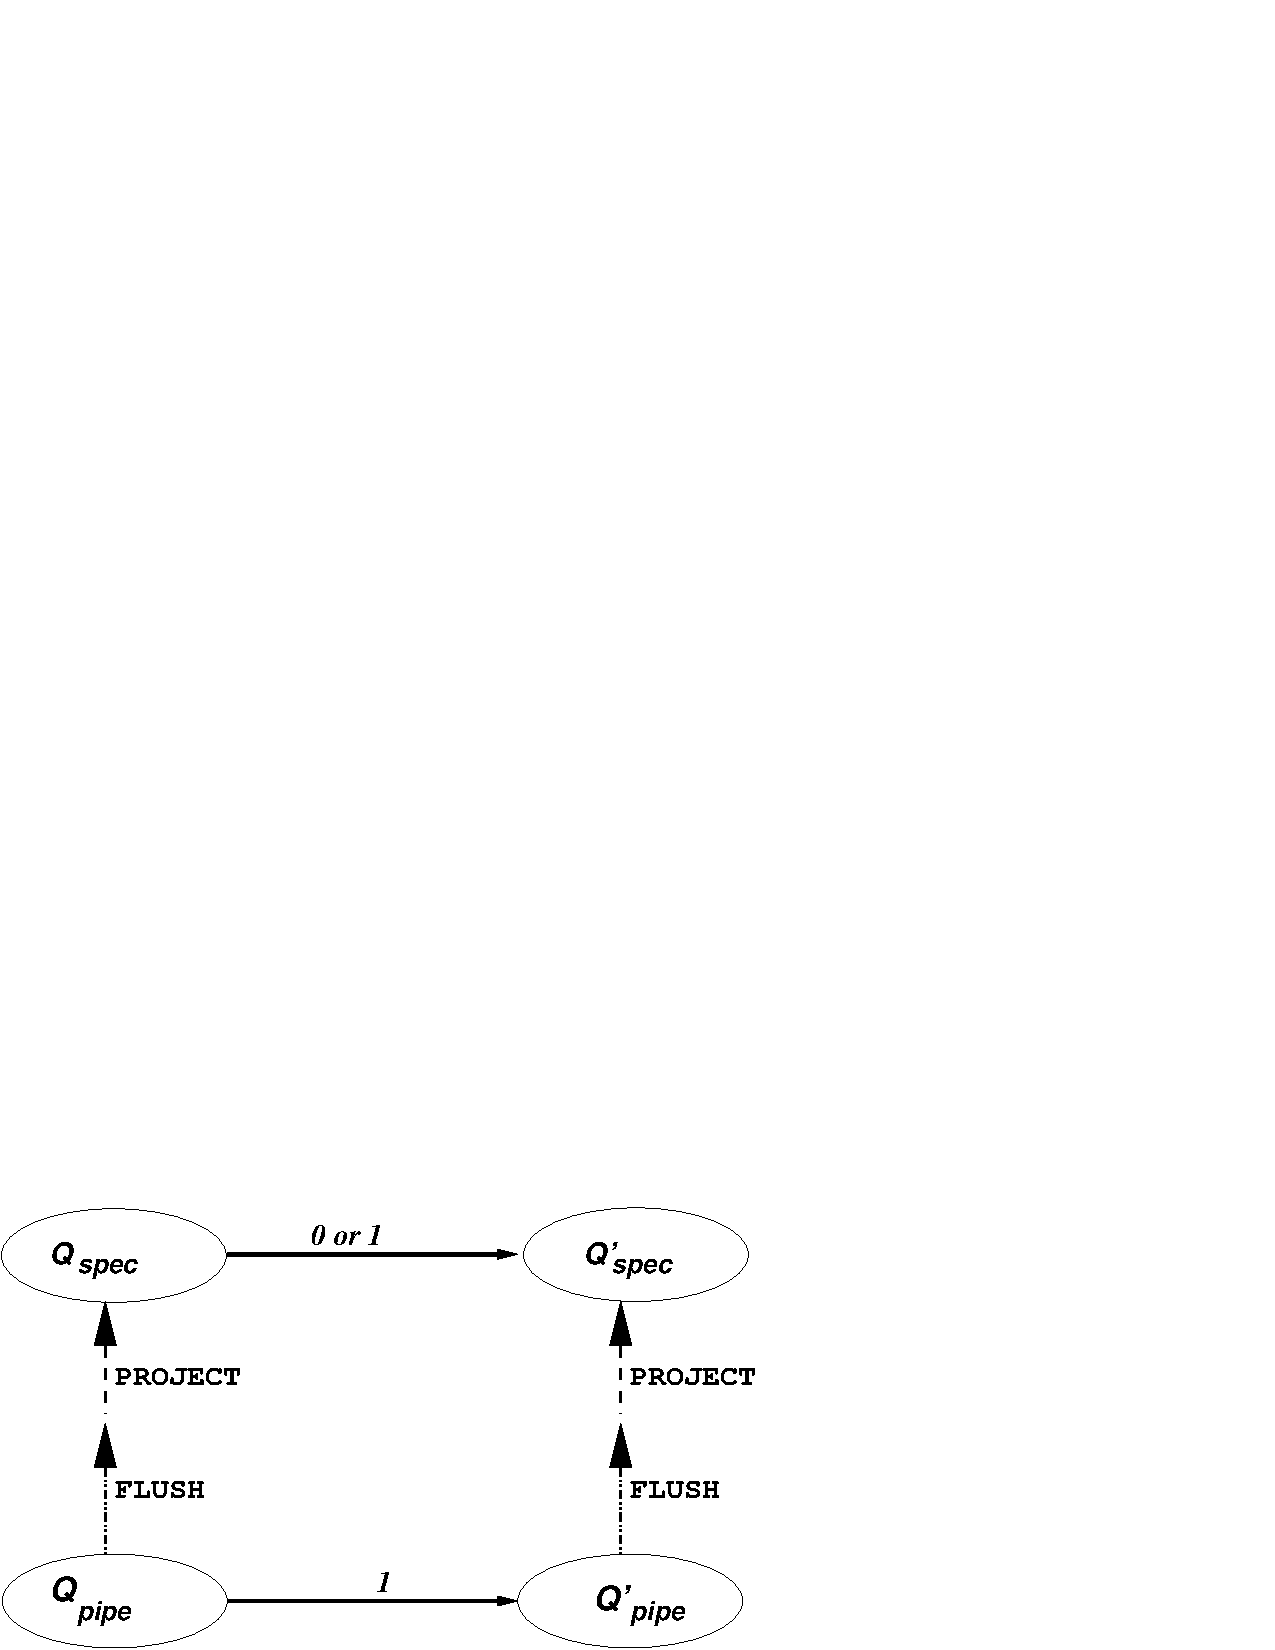
\includegraphics[width=0.7 \columnwidth]{figures/correspond.pdf}
   \label{fig:comm-diag}
	\caption{Commutative diagram to check an implementation (pipelined processor) is simulated by its specification.}
\end{figure}

Thus, the outline of the verification task, as
specified in the control section of a module,
involves simulating the two sides of the commutative (simulation)
diagram and checking an assertion at the end.
An example of correspondence checking, the verification of a simple
pipelined datapath,
is illustrated in detail in the code included below
(also in the distribution in \codelike{examples/simple-datapath.ucl}).
%Example~\ref{ex:simple-datapath}.
This example is drawn from the original UCLID system~\cite{DBLP:conf/cav/LahiriS04,bryant-cav02}.

%\begin{uclidlisting}[htbp]
    \lstinputlisting[language=uclid,style=uclidstyle]{../examples/simple-datapath.ucl}
%    \label{ex:simple-datapath}
%	\caption{\uclid{} model of a simple pipelined datapath in a processor, and verifying that it refines an instruction set architecture (ISA) level model.}
%\end{uclidlisting}


Running \uclid{} on the file given above produces the following output.
%Running \uclid{} on Example~\ref{ex:simple-datapath} produces the following output.

\begin{Verbatim}[frame=single, samepage=true]
$ uclid examples/simple-datapath.ucl
Successfully parsed 4 and instantiated 1 module(s).
10 assertions passed.
0 assertions failed.
0 assertions indeterminate.
Finished execution for module: main.
\end{Verbatim}

%---------------------------------------------------------
\section{Verifying Two-Safety Properties}

Certain security properties involve reasoning about a system
that is composed of modules modeling
multiple interacting agents, some of whom can be malicious. 
For confidentiality
properties, the goal is to ensure that secret data is not revealed to a malicious
agent. For integrity properties, the goal is that actions of a malicious agent
should not be able to influence the values of certain high-integrity variables.
Such properties form a special class of the general category of {\em hyperproperties}~\cite{clarkson-jcs10}
known as {\em $2$-safety properties}. The name arises from the way in which
such properties are checked, by formulating them as a safety property on a
``self-composed'' model of the system --- a model obtained by composing two
copies of the system together synchronously.

With \uclid{}, we verify $2$-safety properties via self-composition and
inductive invariant checking. Counterexamples comprise two traces
and are found by bounded model checking.
The code included below shows an
illustrative \uclid{} model drawn from the chapter on Security from the textbook
on embedded (cyber-physical) systems by Lee and Seshia~\cite{leeseshia-16}.

%\begin{uclidlisting}[htbp]
    \lstinputlisting[language=uclid,style=uclidstyle]{../examples/two-safety.ucl}
%    \label{ex:two-safety}
%	\caption{\uclid{} model of toy problem illustrating verification of two-safety properties}
%\end{uclidlisting}

%---------------------------------------------------------
\section{Synthesis}

\uclid{} has full support for Syntax-Guided Synthesis across all verification modes. If a synthesis function is inserted into the \uclid model, and the control block contains a verification command as per usual, \uclid{} will construct a synthesis query that searches for a body to any synthesis functions in the model. 

The example in Figure~\ref{fig:fib-induction-synth} uses synthesis to strengthen the invariant for the Fibonacci example we have seen before. When run with the command line option \codelike{-y "cvc5 --lang=sygus2"} (or another SyGuS solver), \uclid{} will return the correct body for the synthesis function so that the verification condition passes.

\begin{uclidlisting}[htbp]
    \lstinputlisting[language=uclid,style=uclidstyle]{../examples/fib2safety-synth.ucl}
    \caption{\uclid{} Fibonacci model using \codelike{synthesis function}}
    \label{ex:fib-induction-synth}
\end{uclidlisting}


